\documentclass[11pt, a4paper]{article}

% --- Packages ---
\usepackage{mathptmx} % Sets font to Times Roman 
\usepackage{setspace} % Allows custom line spacing 
\onehalfspacing       % ACTIVATE 1.5 line spacing 
\usepackage[a4paper, margin=1in]{geometry}
\usepackage{natbib} % For APA style citations 
\usepackage{titlesec} % For hierarchical section formatting
\usepackage[hidelinks]{hyperref}
\usepackage{xurl}
\usepackage{parskip} % Use spaces instead of indentation between paragraphs

% --- Graphics Package ---
\usepackage{graphicx}       % Required for including images
\graphicspath{{./}}        % Tell LaTeX to look for images in the main folder
\usepackage{float}

% --- YAML formatting
\usepackage{minted}

% --- Table Package
\usepackage{tabularx}
\usepackage{booktabs}
\usepackage{ragged2e}

\renewcommand*\contentsname{Table of Contents}
\begin{document}

% ==========================================
% FRONT HARD COVER
% ==========================================
\begin{titlepage}
    \centering
    {\Large Undergraduate Research Opportunity Program
(UROP) Project Report\par}
    \vspace*{\fill}
    {\huge \textbf{Design and Implementation of an Observable Global Control Plane for Software-Defined Networks}\par}
    \vspace*{\fill}
    {\Large By\par}
    \vspace{0.5cm}
    {\Large Hon Hao Yuan\par}
    \vspace*{\fill}
    {\Large Department of Computer Science\par}
    {\Large School of Computing\par}
    {\Large National University of Singapore\par}
    \vspace{0.5cm}
    {\Large 2025/2026\par}
\end{titlepage}

% ==========================================
% TITLE PAGE
% ==========================================
\begin{titlepage}
    \centering
    {\Large Undergraduate Research Opportunity Program
(UROP) Project Report\par}
    \vspace*{\fill}
    {\huge \textbf{Design and Implementation of an Observable Global Control Plane for Software-Defined Networks}\par}
    \vspace*{\fill}
    {\Large By\par}
    \vspace{0.5cm}
    {\Large Hon Hao Yuan\par}
    \vspace*{\fill}
    {\Large Department of Computer Science\par}
    {\Large School of Computing\par}
    {\Large National University of Singapore\par}
    \vspace{0.5cm}
    {\Large 2025/2026\par}
    \vspace{1cm}
    \begin{flushleft}
    \large
    Advisor: Assoc Prof Richard Ma Tianbai\par
    \vspace{0.5cm}
    Deliverables:\par
    \qquad \qquad Report: 1 Volume\par
    \end{flushleft}
\end{titlepage}

% --- Front Matter Numbering ---
\pagenumbering{roman}

% ==========================================
% ABSTRACT
% ==========================================
\clearpage
\phantomsection
\addcontentsline{toc}{section}{Abstract}
\begin{center}
    \Large \textbf{Abstract}
\end{center}
\onehalfspacing 

Modern software design has increasingly shifted from monolithic architectures to distributed microservices, offering unparalleled scalability at the cost of system visibility. In these complex environments, understanding the intricate details of service interactions requires robust observability driven by telemetry data: traces, logs, and metrics. This project explores the design and implementation of an enterprise-grade observability and alerting pipeline specifically for the global control plane of a distributed Software-Defined Network (SDN) bandwidth auction system. Abstracting away the underlying data plane, the architecture focuses entirely on the control plane microservices—an API Gateway, an Auction Runner, and a Telemetry stream-processor. The telemetry processor consumes raw network state produced by low-level switches via Kafka, while the entire control plane relies on Atomix for distributed state. By instrumenting these Go services with OpenTelemetry, the system moves beyond basic Kubernetes infrastructure monitoring to capture deep, system-level business health. This precise telemetry is scraped by Prometheus, evaluated against dynamic operational rules, and routed through Alertmanager for real-time Telegram notifications. Ultimately, this project demonstrates how modern observability frameworks can successfully detect "silent failures," dependency outages, and network congestion, ensuring the reliability and economic integrity of distributed SDN control planes.

\vspace{1cm}

\noindent \textbf{Subject Descriptors:}\par
\qquad \qquad C.2.1 Network Architecture and Design \par
\qquad \qquad C.2.3 Network Operations\par
\qquad \qquad C.2.4 Distributed Systems \par
\qquad \qquad D.2.11 Software Architectures \par
\qquad \qquad D.4.5 Reliability

\vspace{0.5cm}

\noindent \textbf{Keywords:}\par
\qquad \qquad Microservices, Observability, OpenTelemetry, Software-Defined Networking, Alerting Systems

\vspace{0.5cm}

\noindent \textbf{Implementation Software and Hardware:}\par
\qquad \qquad Go 1.25.4, Docker, Kubernetes, Minikube 1.37, Kafka 4.1.1, Atomix v0.10.0, Prometheus, Grafana, OpenTelemetry Collector v0.66.0, Jaeger, Loki v13, gRPC v1.78.0

% ==========================================
% ACKNOWLEDGEMENT
% ==========================================
\clearpage % Ensures we start on a fresh page before dropping the anchor
\phantomsection % Drops the invisible hyperlink anchor here
\addcontentsline{toc}{section}{Acknowledgements}

\begin{center}
    \Large \textbf{Acknowledgements}
\end{center}

\onehalfspacing
I would like to sincerely thank my advisor, Prof. Richard Ma, for his continuous support and supervision during this independent project. His willingness to accommodate my academic interests and his clear direction were vital to the project's success. I am deeply grateful for his patience, insightful feedback, and the time he dedicated to our weekly discussions, all of which contributed significantly to my technical and professional growth.

Furthermore, I wish to acknowledge my teammate, Jun Heng, for his valuable technical advice. His insights into system observability and request tracking were highly beneficial during the implementation of the project's infrastructure.

Finally, I am thankful for the opportunity to undertake this project, which has been a deeply rewarding learning experience.
\newpage


% ==========================================
% TABLE OF CONTENTS
% ==========================================
\onehalfspacing 
\tableofcontents
\newpage

\clearpage % Ensures all front matter is printed before saving the number
\newcounter{romanpages} % Creates a custom memory variable
\setcounter{romanpages}{\value{page}} % Saves the current roman page number

% --- Main Report Numbering ---
\pagenumbering{arabic}

% ==========================================
% MAIN REPORT
% ==========================================
\section{Introduction}
\subsection{Background}
Modern enterprise architectures have undergone a significant paradigm shift, transitioning from tightly coupled monolithic systems to distributed microservice architectures. This evolution is particularly evident in modern networking, where Software-Defined Networking (SDN) decouples the network's high-level routing logic (the control plane) from the underlying physical hardware (the data plane).

This project centers on the global control plane of a distributed SDN Internet Exchange Point (IXP) bandwidth auction system. The architecture is composed of several independent Go-based microservices: an \textbf{API Gateway} that enforces policy and handles agent bids, an \textbf{Auction Runner} that acts as the economic engine to continuously clear auctions, and a \textbf{Telemetry Processor} that consumes raw switch counters from the data plane via Kafka. Because these services are distributed, they rely on Atomix—a distributed consensus framework—to maintain shared state, such as bid histories and customer credits. While this microservice approach provides high scalability and fault isolation, it introduces intricate inter-service dependencies that are difficult to monitor.

\subsection{Project Motivation}
As systems become more distributed, the nature of system failures changes. In traditional environments, a failure was often binary: a server crashed, and an alert was triggered. However, in containerized microservice architectures orchestrated by Kubernetes, "silent failures" become a critical risk.

Traditional infrastructure monitoring relies heavily on liveness and readiness probes, which only verify if a Kubernetes pod is running. While Kubernetes is highly effective at detecting hard crashes and restarting failed pods, it is completely blind to business-logic degradation and inter-service congestion. For example, if a critical dependency like the Atomix consensus store experiences severe network congestion or a degraded state, its response times will spike, causing requests to time out. In this scenario, Kubernetes will still report the API Gateway pod as perfectly "healthy" and running because its container has not crashed. The infrastructure looks fine, but the system is silently failing to process incoming bids or read network flows due to the underlying dependency timeouts. Because this project involves an economic system (a bandwidth auction), these silent failures, stalled queues, or dependency chain breaks can lead to severe data inconsistency and financial discrepancies.

Therefore, there is a critical need to move beyond basic infrastructure monitoring. The motivation of this project is to implement "System-Level Health" observability—a framework capable of seeing inside the application code to monitor the success of actual business logic, track the latency and health of inter-service dependencies, and instantly alert human operators when the system degrades, even if the underlying Kubernetes infrastructure appears perfectly healthy.

\subsection{Project Objective}
The primary objective of this project is to design, implement, and validate an enterprise-grade observability and alerting pipeline for the SDN global control plane. To achieve this, the project targets the following specific goals:

\begin{itemize}
    \item \textbf{Instrument Microservices with OpenTelemetry:} Integrate OpenTelemetry—an industry-standard open-source observability framework—into the control plane microservices to generate custom, system-level telemetry. This includes tracking business-specific metrics such as Atomix read/write errors, API policy violations, and Kafka processing throughput.

    \item \textbf{Decouple Telemetry from Application Logic:} Implement fail-safe observability mechanisms (e.g., context timeouts and observable gauges) to ensure that downstream dependency failures do not cause goroutine starvation or crash the primary application threads.

    \item \textbf{Establish a Continuous Monitoring Pipeline:} Deploy and configure Prometheus to continuously scrape the OpenTelemetry Collector, evaluating the incoming metrics against predefined business rules and error thresholds.

    \item \textbf{Implement a Real-Time Alerting Mechanism:} Configure Alertmanager to intercept critical alerts from Prometheus and route them instantly to a network administrator via a Telegram bot.

    \item \textbf{Validate "Silent Failure" Detection:} Prove the efficacy of the pipeline by conducting simulated "soft failures"—such as dependency degradation, network congestion, or database unavailability. The goal is to demonstrate that the custom telemetry successfully detects these business-logic interruptions and triggers appropriate alerts prior to any intervention by infrastructure-level health checks.
\end{itemize}

\section{Technical Background and System Context}

Modern Internet Exchange Points (IXPs) and Software-Defined Networks (SDNs) operate as complex distributed systems where multiple stakeholders compete for shared network resources. Understanding observability in these environments requires grounding in three foundational concepts: (1) the architectural separation between control and data planes, (2) the economic mechanisms that govern resource allocation, and (3) the role of distributed consensus in maintaining system correctness. This chapter provides the technical context necessary to understand why traditional infrastructure-level monitoring (Pod health, CPU usage, network connectivity) is insufficient for detecting business logic failures in control plane systems.

\subsection{Software-Defined Networks and Control Plane Architecture}

\subsubsection{Traditional Network vs. SDN Model}

In conventional networks, forwarding decisions are made by individual network devices (switches, routers) using locally configured policies, making troubleshooting and large-scale policy changes difficult and error-prone. The control plane---the logic that decides \textit{where} traffic goes---is tightly coupled to the data plane---the hardware that actually \textit{forwards} traffic.

Software-Defined Networks decouple these concerns: the data plane (switches) becomes simple forwarding elements, while the control plane runs as a centralized or distributed system making routing decisions. This separation offers significant advantages:

\begin{itemize}
    \item \textbf{Programmability}: Control logic can be defined in software and deployed dynamically
    \item \textbf{Centralized visibility}: A single system has complete knowledge of network state
    \item \textbf{Rapid policy updates}: New rules can be applied instantaneously across the network
\end{itemize}

However, this decoupling introduces a critical observability challenge: \textbf{a failure in the control plane software is invisible to the data plane}. A switch continues forwarding packets normally, even if the control plane has crashed or entered an inconsistent state. From the data-plane perspective, system behavior may still appear healthy.

\subsubsection{The IXP Control Plane}

An Internet Exchange Point control plane must:

\begin{enumerate}
    \item \textbf{Accept resource requests} from member networks (for example, requested bandwidth between specific ingress and egress ports)
    \item \textbf{Allocate resources fairly} according to economic principles or policy rules
    \item \textbf{Update switch policies} in real-time to enforce the allocations
    \item \textbf{Track state consistently} across time and port configurations
    \item \textbf{Report metrics} back to participants so they can adjust their behavior
\end{enumerate}

In a centralized control plane, all five of these functions run in a single service or tightly coordinated set of microservices. If any single function fails---say, the auction engine crashes---the entire system can enter a ``soft failure'' state:

\begin{itemize}
    \item Switches continue forwarding traffic (data plane operational)
    \item Existing network connections remain stable (no dropped packets)
    \item New resource requests cannot be processed (business logic broken)
    \item Pod health checks pass (Kubernetes sees the container running)
    \item Operators may remain unaware of the problem until incident reports are raised
\end{itemize}

This is the core observability challenge that motivates this work.

\subsubsection{Microservices and State Management}

Modern IXP control planes, including the system observed in this project, decompose the monolithic control logic into microservices \citep{babalGrpcMicroservicesGo}:

\begin{itemize}
    \item \textbf{API Gateway}: Accepts bids/requests, enforces authentication, routes to appropriate backend services
    \item \textbf{Auction Runner}: Runs the bandwidth allocation algorithm, computes winners, clearing prices
    \item \textbf{Telemetry Processor}: Consumes data from the physical network, transforms raw metrics into business-level insights
    \item \textbf{Distributed State Store}: Maintains consensus across replicas to ensure consistent state even if nodes fail
\end{itemize}

Each microservice has specialized responsibilities and communicates through a combination of synchronous HTTP REST calls and asynchronous event streams. Specifically:
\begin{itemize}
    \item Customer agents submit bids to the API Gateway via synchronous HTTP REST
    \item The Auction Runner publishes clearing results to Kafka; downstream Local Control Plane components consume these events asynchronously to enforce policies in the data plane
    \item The Telemetry Service ingests flow metrics from Kafka and updates state in Atomix
\end{itemize}

This mixed synchronous/asynchronous architecture provides fault isolation---one service can fail without immediately crashing others---but introduces new observability challenges:

\begin{enumerate}
    \item \textbf{Partial workflow completion}: Multi-step control-plane workflows may complete only some stages (for example, a request is accepted but downstream processing is delayed), creating business-level inconsistency while all pods remain healthy.
    \item \textbf{Dependency instability}: Temporary degradation in external dependencies (state store, message broker, or network path) can increase latency and retry behavior without causing immediate service crashes.
    \item \textbf{Hidden performance degradation}: Services may remain available while response time, queueing delay, and end-to-end completion time gradually worsen, leading to timeouts and missed control-plane deadlines that are invisible to basic health checks.
\end{enumerate}

Observing these systems requires understanding not just whether pods are running, but whether they are correctly processing requests end-to-end \citep{majorsObservabilityEngineering2022}.

\subsection{Bandwidth Auction Mechanisms}

\subsubsection{Economic Motivation}

Bandwidth at an IXP is a shared resource among member networks. Without explicit allocation mechanisms, the network would operate under first-come-first-served or equal-share policies, which may not reflect members' actual demand or willingness to pay.

Auction mechanisms introduce economic efficiency: participants can express their demand and willingness to pay, and the system allocates bandwidth to maximize overall utility or revenue. The specific auction design---uniform-price sealed-bid, Vickrey-Clarke-Groves, or others---determines how fairly and efficiently bandwidth is distributed.

\subsubsection{Sealed-Bid Auction Model}

The system studied in this project uses a periodic sealed-bid auction executed in repeated intervals (rounds):

\textbf{Auction Flow per Interval:}

\begin{enumerate}
    \item \textbf{Bidding Phase}: Customer agents submit bids specifying:
    \begin{itemize}
        \item Ingress port and egress port (if I send traffic from port 60 to port 132...)
        \item Number of bandwidth units (...I want 1000 units...)
        \item Maximum price per unit (...and I'll pay up to 100 SGD per unit)
    \end{itemize}
    
    \item \textbf{Auction Clearing Phase}: Once the bidding window for the interval closes, the auction runner computes the allocation:
    \begin{itemize}
        \item Filter bids by eligibility (customer owns the ingress port)
        \item Sort by price (highest first)
        \item Allocate bandwidth in order until capacity is exhausted
        \item Compute clearing price: the maximum price among winning bids (or a variation thereof)
    \end{itemize}
    
    \item \textbf{Results Distribution}:
    \begin{itemize}
        \item Winners learn their allocation and the clearing price
        \item Losers learn they were not selected
        \item Clearing outcomes are published to Kafka for downstream enforcement
    \end{itemize}
    
    \item \textbf{Switch Policy Updates}:
    \begin{itemize}
        \item The Local Control Plane consumes clearing outputs from Kafka
        \item Updates switch policies in the data plane to enforce allocations
        \item Begins metering traffic to track usage
    \end{itemize}
    
    \item \textbf{Next Interval Begins}: The process repeats with a new bid collection window, creating a continuous interval-based control loop.
\end{enumerate}

\subsubsection{Observability in Auction Systems}

From an observability perspective, a bandwidth auction presents several potential risk patterns that may be inferred from global control-plane signals:

\begin{table}[h]
\centering
\small
\begin{tabularx}{\linewidth}{|l|X|X|}
\hline
\textbf{Potential Issue} & \textbf{Indicative Signal in Global Control Plane} & \textbf{Possible Operational Impact} \\
\hline
Bid intake degradation & API Gateway bid latency or timeout rate rises; bid-write errors to Atomix increase & Some bids may miss the interval window \\
\hline
Auction clearing delay & Auction Runner clearing duration increases, or clearing outputs are delayed & Allocations may be delayed for one or more intervals \\
\hline
Telemetry continuity risk & Telemetry consume/publish counters drop or stop progressing & Control-loop state updates may be delayed or missing for one or more intervals \\
\hline
State-store stress & Atomix read/write latency increases or error rate spikes across services & Cross-service coordination may degrade and deadlines may be missed \\
\hline
\end{tabularx}
\caption{Failure modes in bandwidth auction systems and their observability challenges.}
\label{table:auction_failures}
\end{table}

The listed patterns are conservative and limited to signals observable from the global control plane. They are intended as warning indicators that require correlation with logs, traces, and system context, rather than as definitive proof of root cause.

\subsection{Distributed State Management}

\subsubsection{The Role of Consensus}

In a centralized control plane running on a single server, state is easy to manage: read or write the local database. But a single server is a single point of failure. If that server crashes, the entire control plane is down.

To build a fault-tolerant control plane, the state must be replicated across multiple servers. This introduces a fundamental challenge: if different replicas receive updates at different times, they diverge, and clients may receive inconsistent answers.

\textbf{Distributed consensus} addresses this challenge: it is a protocol that ensures all replicas agree on a single, consistent ordering of updates, even if some replicas crash or network partitions occur.

\subsubsection{Atomix Distributed State Store}

The system studied in this project uses Atomix, an open-source distributed consensus framework. Atomix provides:

\begin{itemize}
    \item \textbf{Replicated maps}: Key-value stores where each write is committed to a distributed log
    \item \textbf{Consensus guarantees}: Writes are persistent and consistent even if nodes fail
    \item \textbf{Strong consistency}: All readers see the same committed values (not ``eventual consistency'')
    \item \textbf{Lean semantics}: Simple get/put operations without complex transactions
\end{itemize}

In this project, Atomix is used as a distributed key-value store. Services use simple \texttt{Put(key, value)} and \texttt{Get(key)} operations over shared maps so control-plane state remains consistent across services.

\subsubsection{Critical Path: Bids $\rightarrow$ Auction Clearing $\rightarrow$ Enforcement}

At a high level, each interval follows a fixed dependency chain: agents read flow state via the API, submit bids, the auction computes allocations, and clearing outputs are propagated for enforcement. The detailed service-by-service sequence is defined in Chapter 3; here the key point is dependency criticality rather than message-level mechanics.

Bid intake and auction computation depend on Atomix being available and correct, while policy enforcement depends on Kafka delivery and the Local Control Plane consumer. If Atomix:

\begin{itemize}
    \item Becomes unavailable (partition, all replicas down): Control plane cannot read or write state $\rightarrow$ entire system halts
    \item Has replication lag (slow network): Auction clearing may read incomplete bid state within interval deadlines $\rightarrow$ wrong allocations
    \item Has bugs in consensus protocol: Replicas diverge $\rightarrow$ different views of port allocation
\end{itemize}

From the perspective of pod health checks, Atomix pods may appear ``Running'', yet if the consensus protocol is stuck, the system is functionally broken.

\subsubsection{Failure Modes in Distributed Systems}

Distributed control planes introduce failure modes that are often \textit{degradations} rather than crashes:

\begin{itemize}
    \item \textbf{Partitioned connectivity}: replicas remain running but cannot coordinate reliably.
    \item \textbf{Inconsistent progress}: parts of a workflow complete while downstream steps stall.
    \item \textbf{Slow consensus path}: write and read latency rises, delaying control decisions.
\end{itemize}

These conditions usually pass basic health checks, but they can still break business correctness.

\subsection{The Observability Gap: Hard Crashes vs. Soft Failures}

\subsubsection{Hard Failures (Kubernetes-Visible)}

A \textbf{hard failure} is complete service unavailability (for example, process crash or OOM kill). Kubernetes already handles this well through probes, restarts, and scheduling.

\subsubsection{Soft Failures: Congestion and Latency (Invisible to Kubernetes)}

A \textbf{soft failure} occurs when services remain \texttt{Running} but fail to meet timing and correctness expectations. Typical symptoms are increased latency, queue buildup, delayed state propagation, and request timeouts across dependent services.

\subsubsection{Why Kubernetes and Standard Metrics Cannot Detect Congestion Failures}

Kubernetes probes check \textit{availability}, not \textit{performance}:

\begin{itemize}
    \item \textbf{Liveness probe}: confirms process survival, not request quality.
    \item \textbf{Readiness probe}: confirms basic reachability, not end-to-end deadline compliance.
\end{itemize}

Traditional infrastructure metrics also miss congestion failures:

\begin{itemize}
    \item \textbf{CPU and memory}: may look normal while requests still queue or timeout.
    \item \textbf{Network throughput}: does not reveal whether control decisions arrive in time.
\end{itemize}

\subsubsection{The Root Cause: Dependency Chain Latency}

The critical path for each auction interval is latency-sensitive at multiple steps:

\begin{enumerate}
    \item Customer agent fetches /flows endpoint (depends on: Telemetry Service latency in Atomix)
    \item Customer agent submits bid (depends on: API Gateway latency + Atomix write latency)
    \item Auction Runner computes clearing (depends on: reading all bids from Atomix)
    \item Auction Runner publishes clearing outputs to Kafka (depends on: broker availability + publish latency)
    \item Telemetry pipeline refreshes flow state for the next interval (depends on: Kafka consumption + Atomix write latency)
\end{enumerate}

If one step slows down, downstream steps accumulate delay. The system may remain available but still violate control-plane deadlines and service expectations.

\subsubsection{Observability Requirements as Design Goals}

Not every failure condition can be tested in one evaluation. For this reason, the observability requirements in this project are presented as design goals. These goals describe the evidence needed to detect and diagnose soft failures along the critical path:

\begin{enumerate}
    \item \textbf{Per-operation latency metrics}:
    \begin{itemize}
        \item Time to write bid to Atomix (latency percentiles: p50, p95, p99)
        \item Time to read flows from Atomix
        \item Time for Auction Runner to clear (from all bids received to results written)
        \item Time for telemetry updates to persist flow state (from Kafka message to Atomix write)
    \end{itemize}
    
    \item \textbf{Request timeout and error monitoring}:
    \begin{itemize}
        \item Timeout rate and failure rate per operation type
        \item Alerts when thresholds indicate potential service-objective violations
    \end{itemize}
    
    \item \textbf{Dependency health indicators}:
    \begin{itemize}
        \item Atomix read/write latency
        \item Kafka publish and consumer lag
        \item Telemetry flow-update continuity used by agents
    \end{itemize}
    
    \item \textbf{End-to-end control-loop visibility}:
    \begin{itemize}
        \item Total time from bid submission to clearing publication and observable state update
        \item Bottleneck localization when one stage appears to degrade
    \end{itemize}
\end{enumerate}

\subsection*{Summary}

The bandwidth auction control plane is a distributed system where:

\begin{itemize}
    \item \textbf{Control and data planes are decoupled}: Failures in the control plane are invisible to the data plane (the switch continues forwarding).
    \item \textbf{Consensus-based state management}: Relies on Atomix to maintain a consistent view across multiple replicas; failures here are not obvious (all replicas may appear healthy but diverge).
    \item \textbf{Asynchronous processing}: Auction and telemetry pipelines exchange events through Kafka; failures may be delayed or silent.
    \item \textbf{Economic contracts}: Business correctness depends on all steps of the auction proceeding correctly; partial execution leads to SLA violations without visible symptoms.
\end{itemize}

Traditional Kubernetes-level observability (pod health, CPU, memory) is insufficient because it primarily detects hard failures. Soft failures---where the control plane may violate timing or correctness expectations despite appearing healthy---require business-aware instrumentation: metrics, traces, logs, and alerts that provide evidence of system behavior rather than process availability alone.

Chapter 4 presents an application-level observability framework for auction, state-store, and telemetry paths. In evaluated scenarios, it improved incident visibility and diagnosis; broader validation remains future work.


\section{System Design and Architecture}

This chapter describes the system architecture used in this project. The main focus is the \textbf{global control plane} and the telemetry around it. The local control plane and data plane are treated as external boundaries: they are part of the full system, but they are not instrumented in this project.

\subsection{High-Level Architecture Overview}

The system is organized into three parts:

\begin{itemize}
    \item \textbf{Global control plane}: API Gateway, Auction Runner, Telemetry Processor, and shared state managed by Atomix.
    \item \textbf{Local control plane (external boundary)}: consumes clearing outputs and applies enforcement decisions toward switch-facing functions.
    \item \textbf{Data plane (external boundary)}: physical switching and metering behavior that produces traffic counters.
\end{itemize}

\begin{figure}[h]
    \centering
    \IfFileExists{fyp-full-architecture.pdf}{
        \includegraphics[width=0.95\linewidth]{fyp-full-architecture.pdf}
    }{
        \fbox{\parbox{0.9\linewidth}{\centering
        Placeholder for the full relevant FYP architecture diagram.\\
        }}
    }
    \caption{Full system architecture of the Software Defined Network (SDN) bandwidth auction platform}
    \label{fig:fyp-full-architecture}
\end{figure}

Within project scope, this chapter covers the part of the system we observe: bids, auctions, shared state, and the flow and account data served to agents.

The services communicate in three ways:

\begin{itemize}
    \item \textbf{Synchronous REST}: customer agents call API endpoints for bids, credits, auction snapshots, and flow reads.
    \item \textbf{Asynchronous events via Kafka}: the Auction Runner publishes clearing outputs to Kafka, and the Telemetry Processor consumes telemetry messages from Kafka.
    \item \textbf{Shared state via Atomix}: the services read and write shared maps to keep state aligned.
\end{itemize}

This split keeps responsibilities separate, but a slow service can still delay the rest of the control loop without causing a hard crash.

\subsection{Control Plane Microservices}

\subsubsection{API Gateway (Control Plane Ingress and Policy Enforcement)}

The API Gateway is the entry point for control-plane requests. It validates bid submissions, serves flow and credit data, and reads and writes shared state.

Because all agents pass through this service, it is where congestion and timeout issues show up first.

\subsubsection{Auction Runner (Economic Engine)}

The Auction Runner runs once per interval. It reads bids from Atomix, applies the auction algorithm, computes allocations and clearing prices, writes credits, utility, and auction history back to Atomix, clears the bid map, and publishes clearing outputs to Kafka.

Its role is deterministic economic decision-making under time constraints:

\begin{itemize}
    \item \textbf{Input}: current-interval bids and static scenario constraints (capacity, eligibility, reservation logic).
    \item \textbf{Computation}: sort/filter and allocate according to auction rules.
    \item \textbf{Output}: clearing results and per-interval state updates for downstream consumers.
\end{itemize}

From a systems perspective, this component sets the pace of the control loop. If clearing slows down, the next interval starts later.

\subsubsection{Telemetry Processor (Data Plane Bridge via Kafka)}

The Telemetry Processor reads telemetry messages from Kafka, computes flow metrics, and writes the latest flow state to Atomix. This keeps the current flow data available to the API Gateway and agents.

Its core responsibilities are:

\begin{itemize}
    \item \textbf{Stream ingestion}: consume telemetry messages from Kafka topics.
    \item \textbf{State transformation}: derive flow metrics from raw event streams.
    \item \textbf{State publication}: write the computed flow state into shared storage for API reads.
\end{itemize}

This service keeps the latest flow data available for later bidding rounds.

\subsubsection{Distributed State Store (Atomix Integration)}

Atomix stores the shared state for the global control plane. The project uses shared maps for bids, auction outputs, flow values, credits, utility, and auction history.

Operationally, these shared maps are used as key-value stores. Services write state with operations equivalent to \texttt{put(key, value)} and retrieve state with \texttt{get(key)}, where keys represent control-plane entities (for example flow identifiers, auction interval keys, or customer IDs) and values hold the latest committed state. This key-value access pattern keeps inter-service coordination simple and predictable.

The design rationale is operational correctness under distributed execution:

\begin{itemize}
    \item \textbf{Single logical source of truth}: services read the same committed state.
    \item \textbf{Cross-service coordination}: API, auction, and telemetry paths share the same data structures.
    \item \textbf{Failure tolerance}: replicated state reduces dependence on a single node.
\end{itemize}

Because many critical operations use Atomix, its latency affects the whole control loop.

\subsection{Data and Event Flow Model}

The system behavior can be summarized as three interacting data and event paths.

\textbf{Path A: Bid Ingestion and Clearing}

\begin{enumerate}
    \item Customer agents submit bids through the API.
    \item API Gateway validates and persists bid data to Atomix.
    \item Auction Runner reads interval bids from shared state.
    \item Auction Runner computes allocation and clearing price.
    \item Clearing outputs are published to Kafka for downstream consumers.
\end{enumerate}
\textbf{Path B: Telemetry Update Path}

\begin{enumerate}
    \item Telemetry messages are ingested from Kafka.
    \item Telemetry Processor derives flow metrics.
    \item Updated flow state is written to Atomix.
    \item API Gateway serves the refreshed values to agents.
\end{enumerate}

\textbf{Path C: Agent Decision Interaction}

\begin{enumerate}
    \item Agents read the latest flow and auction data.
    \item Agents compute next bids using their strategy.
    \item Updated bids are submitted through the API path.
\end{enumerate}

Together, these paths show how requests, state updates, and telemetry move through the global control plane.

\subsection{Architecture Boundaries and Project Scope}

To avoid overstating implementation coverage, this report distinguishes between observed and non-observed domains:

\begin{itemize}
    \item \textbf{In scope}: global control-plane services and their interfaces (API Gateway, Auction Runner, Telemetry Processor, Atomix integration, Kafka interactions from these services).
    \item \textbf{Out of scope}: direct instrumentation of local control plane enforcement logic and data-plane switch internals.
\end{itemize}

Accordingly, later chapters focus on detecting degradation in the global control-plane loop and giving early warnings to operators. They do not claim full visibility into downstream enforcement internals.


\section{Observability Framework Design}

This chapter presents the observability framework designed for the SDN global control plane introduced in Chapter 3. The framework is built to detect soft failures early, localize likely fault domains, and support operator decision-making during live auction intervals. The focus is not infrastructure uptime alone, but correctness and timeliness of control-plane behavior \citep{majorsObservabilityEngineering2022}.

\subsection{Design Goals and Scope}

The design was guided by four practical goals:

\begin{itemize}
	\item \textbf{Business-level visibility}: expose auction and control-path health signals that directly reflect system outcomes, not only container health.
	\item \textbf{Fast degradation detection}: surface warning signs (rising latency, growing error rates, telemetry interruption) before complete request failure.
	\item \textbf{Low operational coupling}: ensure telemetry collection does not become a source of cascading failure in request-critical code paths.
	\item \textbf{Actionable alerts}: route concise, severity-scoped alerts to operators with enough context for triage.
\end{itemize}

The observability boundary remains consistent with project scope and follows Chapter 3's architecture model: API depends on Atomix, Auction spans Atomix and Kafka, and Telemetry bridges Kafka to Atomix.

\subsection{Control-Plane Observability Model}

The framework uses three complementary signal classes:

\begin{itemize}
	\item \textbf{Service availability signals}: request success/failure and API error-rate trends.
	\item \textbf{Dependency-chain signals}: Atomix operation failure counters and categorized error types (for example timeout and connection errors).
	\item \textbf{Congestion and telemetry continuity signals}: percentile latency growth and telemetry publication continuity.
\end{itemize}

To support consistent rule design, these signals are mapped to practical service-level indicators rather than strict closed-form formulas. In implementation, the alerts look for patterns such as falling success rates, increasing dependency errors, and sustained latency growth over a time window.

This approach favors interpretability over mathematical precision, which is more appropriate for operational alerting because the underlying signals are threshold-based and may combine multiple conditions before firing.

While service-level indicators (SLIs) are primarily metric-based for threshold evaluation, the framework is intentionally tri-modal: metrics are used for detection, traces for causal path reconstruction, and logs for event-level evidence.

\subsection{Why OpenTelemetry: Strategic Choice and Trade-offs}

A central design question is whether a traditional observability approach---using only logs, a single metrics library, or proprietary application performance monitoring (APM) agents---would suffice. The answer depends on whether the system requires multi-service correlation and long-term operational flexibility.

\textbf{Without unified instrumentation}, each service would emit signals via different paths: application logs to Loki, custom metrics to Prometheus, and traces (if any) via direct instrumentation. The result is fragmentation: a request failure might trigger a metric alert, but drilling into the cause requires hypothesis-driven log searches and manual span correlation across services. This becomes expensive operationally when an incident spans the API Gateway, Auction Runner, and Telemetry Processor.

\textbf{OpenTelemetry's unified SDK} addresses this cost directly. By standardizing on a single instrumentation point per service (the OTel SDK), the framework guarantees \citep{youngLearningOpenTelemetry2023,opentelemetryDocsOverview}:

\begin{itemize}
	\item \textbf{Vendor neutrality}: Exporters can be swapped (from Prometheus to any backend) without re-instrumenting code, reducing technical debt and lock-in over the thesis runtime and beyond.
	\item \textbf{Trace context propagation}: Spans automatically link across service boundaries via context headers, enabling end-to-end causal reconstruction without manual trace ID plumbing.
	\item \textbf{Signal correlation}: A single tracing failure carries both a metric error counter and log evidence without explicit coordination between detection and verification systems.
	\item \textbf{Minimal request-path impact}: Non-blocking metric recording and bounded context deadlines keep observability from becoming a bottleneck.
\end{itemize}

The operational cost is twofold: integration effort (writing metric instruments and span boundaries in code) and collector overhead (CPU and memory for the centralized OpenTelemetry Collector). For a three-service control plane with bounded cardinality and short request windows, this cost is justified because it compresses troubleshooting time from hypothesis-driven log searches to seconds of trace visualization and alert navigation.

This choice also improves reproducibility for the evaluation chapter: alert-firing scenarios (Atomix degradation, Kafka congestion) can be validated against a single unified metric stream rather than correlating logs and metrics in an ad-hoc manner.

\subsection{Instrumentation Strategy}

\subsubsection{Metrics, Traces, and Logs Coverage}

The instrumentation strategy is designed as a layered signal model rather than a metrics-only model \citep{majorsObservabilityEngineering2022}:

\begin{itemize}
\item \textbf{Metrics (continuous health signals)}: time-series indicators used for trend monitoring and alert triggering. In line with OpenTelemetry guidance, they should be defined carefully because high-cardinality or high-frequency metrics can become expensive to collect and export \citep{opentelemetryDocsMetricsBestPractices}.
\item \textbf{Traces (request path context)}: span-level timing and dependency visibility across API, auction, telemetry, Atomix, and Kafka interactions.
\item \textbf{Logs (event evidence)}: structured runtime records for errors, retries, and edge-case behavior that may not be fully captured by counters and histograms.
\end{itemize}

This separation allows each signal to serve a distinct operational function: detect, localize, and verify.

In particular, the framework treats business-logic metrics as early-warning indicators of control-plane degradation. Counters such as auction intervals completed without bids or Atomix operation failure rates can surface anomalies before a full service outage occurs, while traces and logs provide the causal evidence needed to localize and verify the underlying issue.

\subsection{Observability Architecture Overview}

The observability architecture is centered on the three in-scope Go services in the global control plane: the API Gateway, the Auction Runner, and the Telemetry Processor. Each service emits OpenTelemetry signals from application code, with the API Gateway and Auction Runner focusing on request health, dependency failures, and latency, while the Telemetry Processor additionally tracks Kafka consumption and Atomix write behavior.

These signals are collected by a shared OpenTelemetry Collector, which exports metrics to Prometheus for rule evaluation, traces to Jaeger for causal analysis, and logs to Loki for event-level inspection. Prometheus alert rules then evaluate the exported metrics and forward incidents through Alertmanager to Telegram.

The architecture is intentionally scoped to the observability pipeline rather than the full SDN topology. The data plane and local control-plane enforcement logic remain external actors, while the diagram concentrates on how telemetry moves from the instrumented services into alerts.

\begin{figure}[htbp]
	\centering
	\IfFileExists{observability-architecture.pdf}{
		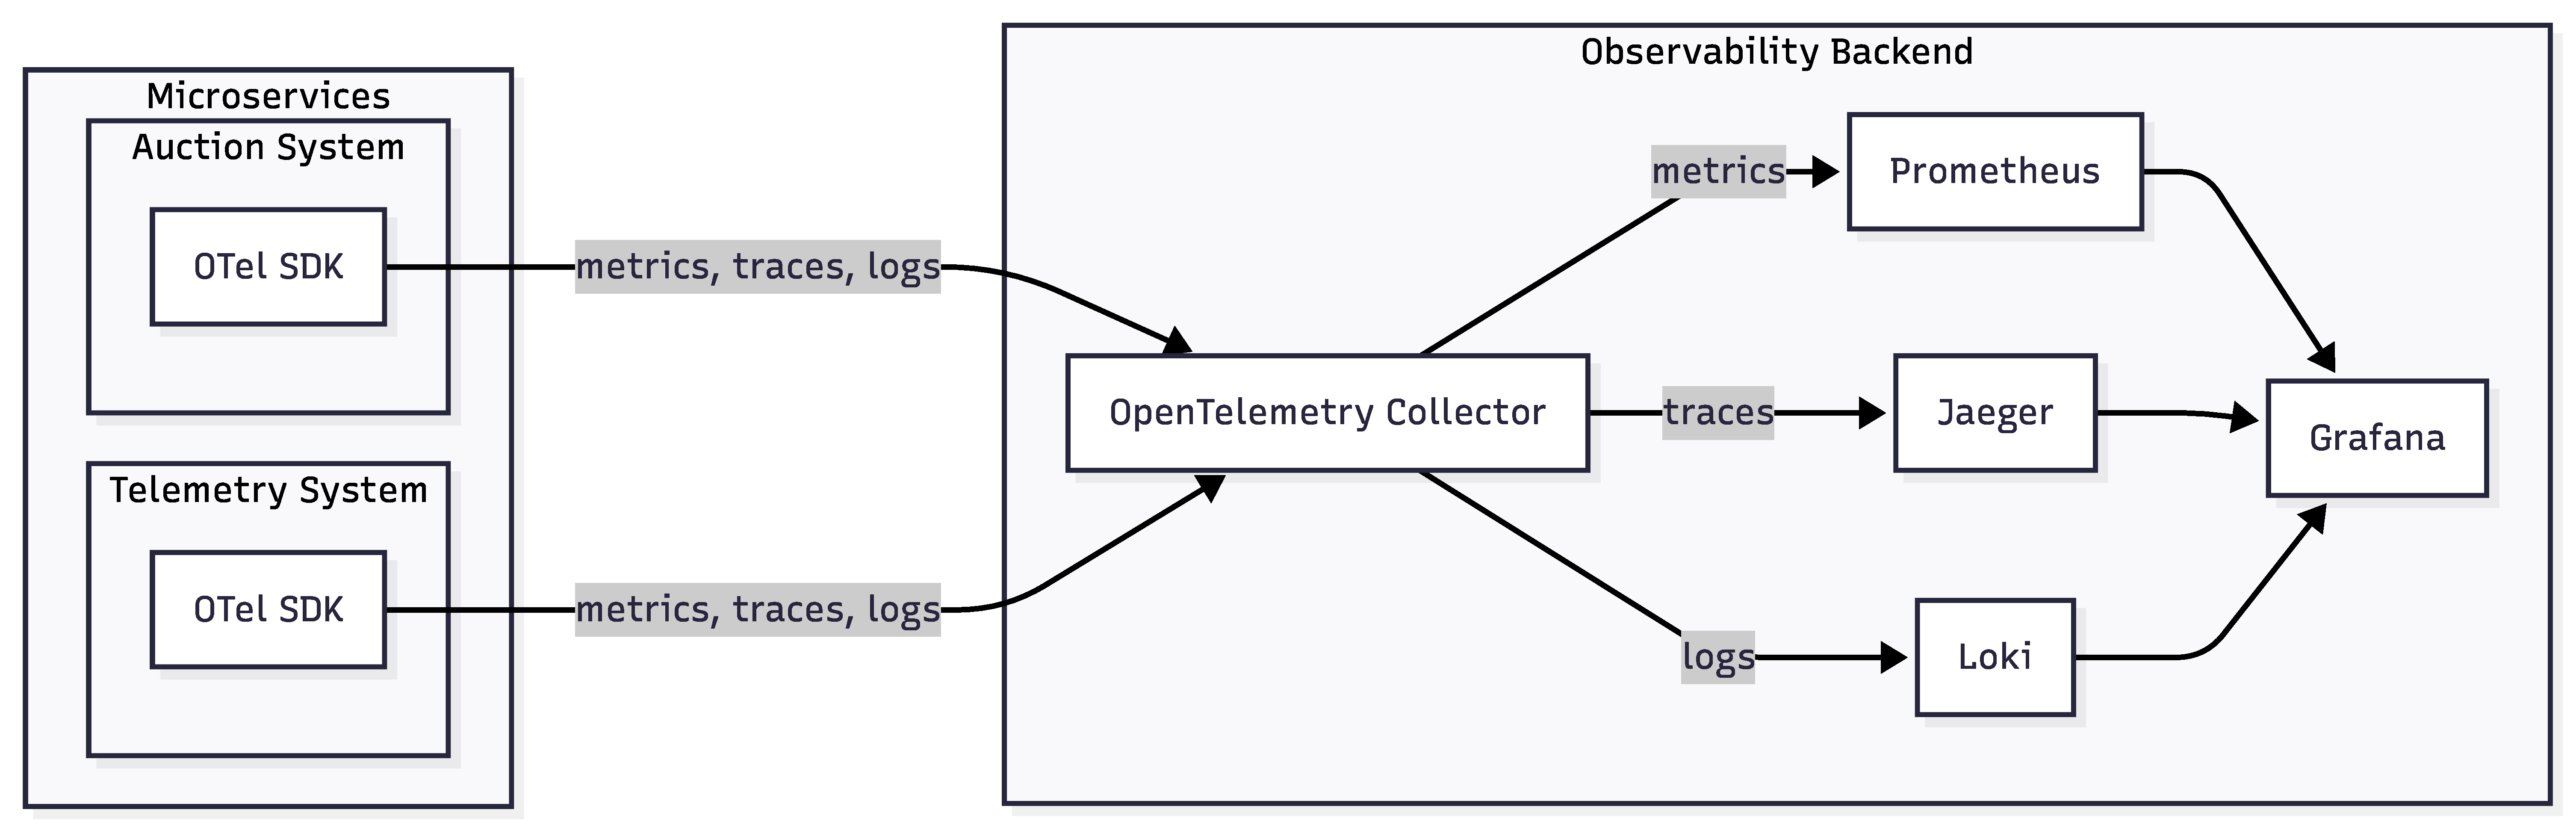
\includegraphics[width=0.95\linewidth]{observability-architecture.pdf}
	}{
		\fbox{\parbox{0.9\linewidth}{\centering
		Mermaid source for this architecture is stored in \texttt{observability-architecture.mmd}. Render it to a PDF and place it in the report folder to include the figure here.
		}}
	}
	\caption{OpenTelemetry-based observability architecture for the global control plane}
	\label{fig:observability-architecture}
\end{figure}

\subsubsection{OpenTelemetry Integration Pattern}

All in-scope microservices are instrumented with OpenTelemetry SDKs and export telemetry through OTLP to a centralized OpenTelemetry Collector. Instrumentation is designed around these conventions \citep{youngLearningOpenTelemetry2023,opentelemetrySpecOTLP}:

\begin{itemize}
	\item domain-prefixed metric instruments (for example, \texttt{ixp.auction.*}, \texttt{ixp.api.*});
	\item stable label sets to avoid excessive time-series cardinality;
	\item explicit units (for example \texttt{kbps}, \texttt{SGD}, \texttt{ms}) for alert consistency;
	\item graceful shutdown flushing to reduce metric loss during rollout and restart events.
\end{itemize}

Metrics are transformed by the collector and Prometheus naming rules (dots to underscores, unit suffixes, and counter \texttt{\_total} suffixes).

\subsubsection{Spans and Distributed Context}

Two foundational concepts underpin distributed tracing: \textbf{spans} and \textbf{context}. Understanding their roles is essential for interpreting the implementation code in Chapter 5.

A \textbf{span} is an atomic unit of work or operation within a service. It has a name, start time, end time, and status (success or failure). Each span may contain semantic attributes (such as operation type, component name, or request ID) that provide meaning without requiring human interpretation of timestamps alone. Spans form a directed acyclic graph: a parent span represents a higher-level operation and may have child spans representing sub-operations or dependency calls. For example, an API Gateway request handler is a parent span, and a call to Atomix for state lookup is a child span.

A \textbf{trace} is the full chain of related spans that together represent one end-to-end unit of work across a system. In practical terms, a trace begins with a root span and then collects all child spans created while the request moves through the API Gateway, Auction Runner, Telemetry Processor, and any dependency calls. This is why a single trace can contain multiple spans: each span records one step in the work chain, while the trace captures the entire causal path from start to finish.

A \textbf{distributed context} (or trace context) is the metadata that flows alongside a request as it propagates across service boundaries. It contains the trace ID (unique identifier for the entire request's journey) and span ID (identifier for the current span), allowing a child service to link its spans back to the parent service's request. Context is typically transmitted in request headers (HTTP, gRPC, or Kafka message headers) so that the observability backend can reconstruct the causal chain even when services are geographically or temporally decoupled \citep{w3cTraceContext,opentelemetryDocsContextPropagation}.

In practical terms, when the API Gateway receives a bid and calls Atomix to check policy constraints, the trace context is extracted at API ingress and a client-side dependency span is recorded around the outbound Atomix call. In this project, Atomix is treated as an external black-box dependency and is not instrumented internally, so traces show only the control-plane service spans plus client-side dependency timing from the caller perspective.

The framework uses context for two distinct purposes:
\begin{itemize}
	\item \textbf{Trace propagation}: preserving the trace ID across service calls so spans can be linked in the observability backend.
	\item \textbf{Timeout and cancellation}: golang contexts carry deadlines and cancellation signals, allowing bounded operations that fail fast if dependencies time out.
\end{itemize}

Both purposes are important: the first enables causal debugging, the second prevents resource exhaustion when upstream services are unavailable.

\subsubsection{Distributed Tracing Design}

Trace instrumentation uses span boundaries at request entry, dependency calls, and asynchronous hand-off points. The objective is to reconstruct end-to-end control-path timing for each interval cycle and identify where latency is introduced.

One important design detail in this project is that bid-ingress tracing and auction-execution tracing do not share a single synchronous call chain. Bid spans are created in request-time API handlers, while auction spans are created later in interval-driven runner execution. Because these spans are produced in different execution contexts, direct parent-child continuity is not always available across the shared-state boundary.

Key tracing design choices are:

\begin{itemize}
\item parent-child span structure across in-scope control-plane services, with client-side dependency spans for external systems;
\item semantic span attributes (operation type, component, and key identifiers such as ingress or egress context where appropriate);
\item span-link based correlation for asynchronous bid write to auction read handoff, using propagated trace context in shared store payloads;
\item consistent propagation of context to preserve causal linkage across services.
\end{itemize}

Traces are exported through the OpenTelemetry Collector to Jaeger, where operators can inspect critical-path delay and dependency bottlenecks.

\subsubsection{Structured Logging Design}

Structured logs are emitted with stable keys (service, operation, error class, and contextual identifiers) so that they can be queried reliably in aggregation backends.

The logging layer focuses on evidence that complements metrics and traces:

\begin{itemize}
\item explicit dependency errors (for example timeout, connection, and unavailable states);
\item state-transition events (for example bid handling outcomes and telemetry publication results);
\item recovery and retry behavior during transient failures.
\end{itemize}

Logs are exported through the collector to Loki, enabling timeline-based correlation with alerts and traces during incident analysis.

\subsubsection{Decoupling Telemetry from Request-Critical Paths}

A critical design principle is that the observability infrastructure itself must not become a source of failure. Per the OpenTelemetry error-handling specification, SDKs must handle their own failures gracefully without destabilizing application logic \citep{opentelemetrySpecErrorHandling}.

The framework implements two core safeguards:

\begin{itemize}
	\item \textbf{SDK error handler registration}: Each service registers a custom error handler that logs SDK failures (exporter unavailability, context propagation errors, metric overflow) without affecting request processing. This allows operators to diagnose observability-stack problems independently from application behavior.
	\item \textbf{Non-blocking telemetry patterns}: Bounded context deadlines, non-blocking metric recording, and defensive error classification (timeout, connection, not found, other) ensure that transient observability-collector unavailability does not propagate as user-facing errors.
\end{itemize}

These patterns ensure that when the observability pipeline itself degrades, the control plane remains operational while the SDK error logs surface the infrastructure problem for remediation.

\subsection{Monitoring and Alerting Architecture}

\subsubsection{Collector and Storage Pipeline}

The telemetry data path is structured as follows:

\begin{enumerate}
	\item Services emit OpenTelemetry Protocol (OTLP) telemetry to the OpenTelemetry Collector.
	\item The collector applies memory-limit and batching processors.
	\item Metrics are exported for Prometheus scraping.
	\item Traces are exported to Jaeger.
	\item Logs are exported to Loki.
	\item Prometheus evaluates alert rules on fixed intervals.
	\item Alertmanager groups, deduplicates, and routes alerts to Telegram.
\end{enumerate}

This centralized pipeline decouples application instrumentation from backend storage and notification concerns while preserving cross-signal correlation.

\subsubsection{Alert Rule Taxonomy}

Alert rules are grouped by failure semantics rather than by component ownership:

\begin{itemize}
	\item \textbf{Availability alerts}: reduced API success rate.
	\item \textbf{Dependency-chain alerts}: increasing Atomix operation errors and near-total failure conditions.
	\item \textbf{Congestion alerts}: sustained p50/p95/p99 latency elevation on critical operations.
	\item \textbf{Telemetry continuity alerts}: low or absent flow publication despite expected system activity.
\end{itemize}

This taxonomy improves operator triage by reflecting likely incident phases: early slowdown, partial failure, then widespread service impact. In practice, metric alerts trigger first, traces identify delayed segments, and logs provide root-cause evidence.

\subsubsection{Severity Mapping and Notification Policy}

To reduce alert fatigue while preserving responsiveness, rule severities are staged:

\begin{itemize}
	\item \textbf{Warning}: early anomalous behavior that may self-recover but should be watched.
	\item \textbf{Critical}: probable service impact requiring prompt intervention.
\end{itemize}

Alertmanager routes notifications to Telegram with labels and annotations describing likely cause, affected path, and suggested first checks.

\subsection{Summary}

The resulting framework combines metric semantics, distributed tracing, structured logging, rule design, and operator workflow into one control-plane observability system. Its design emphasis is early warning for soft failures and actionable incident triage, preparing the ground for the implementation details and evaluation scenarios in the next chapters.


\section{Implementation Details}

This chapter describes how the observability framework is implemented in the global control plane, focusing on instrumentation, alerting components, and deployment resources. Evaluation outcomes are deferred to the next chapter.

\subsection{Implementation Scope}

Implementation scope mirrors Chapter 3 boundaries: API Gateway, Auction Runner, and Telemetry Processor are instrumented; local-control-plane enforcement and data-plane internals remain external.

\subsection{Go Microservice Instrumentation}

The instrumentation is implemented in a shared bootstrap layer and then consumed consistently by each service entry point. Instead of duplicating setup logic per service, the code uses \texttt{shared/otel/otel.go} and \texttt{shared/otel/otel-init.go} as the common initialization path, aligned with the OpenTelemetry Go instrumentation guidance at \url{https://opentelemetry.io/docs/languages/go/instrumentation/} \cite{opentelemetryGoInstrumentation} and informed by the OpenTelemetry demo patterns at \url{https://opentelemetry.io/docs/demo/} \cite{opentelemetryDemo}.

\subsubsection{Shared OpenTelemetry Bootstrap (\texttt{otel.go})}

The shared bootstrap configures OTLP exporters for traces, metrics, and logs, registers global providers, and returns a shutdown function used by all services.

\begin{minted}[fontsize=\small,breaklines]{go}
func SetupOTelSDK(ctx context.Context) (func(context.Context) error, error) {
    endpoint := os.Getenv("OTEL_EXPORTER_OTLP_ENDPOINT")
    if endpoint == "" {
        endpoint = "localhost:4317"
    }

    tracerProvider, _ := newTracerProvider(endpoint)
    otel.SetTracerProvider(tracerProvider)

    meterProvider, _ := newMeterProvider(endpoint)
    otel.SetMeterProvider(meterProvider)

    loggerProvider, _ := newLoggerProvider(endpoint)
    global.SetLoggerProvider(loggerProvider)

    return shutdown, err
}
\end{minted}

The implementation uses a short periodic metric export interval and a timeout-bounded exporter setup to reduce startup hangs and make observability behavior easier to debug during development.

\subsubsection{Shared Instrument Binding (\texttt{otel-init.go})}

After SDK setup, the code binds package-level logger, tracer, and meter handles to the active service name so each service emits under a stable identity.

\begin{minted}[fontsize=\small,breaklines]{go}
var (
    Logger *slog.Logger = slog.Default()
    Tracer trace.Tracer = otel.Tracer("ixp-default")
    Meter  metric.Meter = otel.Meter("ixp-default")
)

func InitInstruments() {
    serviceName := os.Getenv("OTEL_SERVICE_NAME")
    if serviceName == "" {
        serviceName = "ixp-service"
    }
    Logger = otelslog.NewLogger(serviceName)
    Tracer = otel.Tracer(serviceName)
    Meter = otel.Meter(serviceName)
    slog.SetDefault(Logger)
}
\end{minted}

\subsubsection{Service Startup Pattern Across API, Auction, and Telemetry}

All three services follow the same startup sequence: initialize the OpenTelemetry SDK, bind the service-scoped instruments, register domain metrics, register dependency metrics, and then defer shutdown flushing. The key implementation point is not the boilerplate itself, but the fact that observability is initialized before request handling or message processing begins. This keeps the service startup order consistent while matching each service's actual dependencies: the API Gateway tracks Atomix; the Auction Runner tracks Atomix and Kafka; and the Telemetry Processor tracks Kafka and Atomix.

\subsubsection{General Tracing and Logging Implementation Pattern}

To keep observability balanced across signals, each critical operation follows a repeatable trace-and-log pattern: start a span, execute the dependency call with a bounded context, record span status, emit a structured error log on failure, and end the span. The same pattern is applied at API handlers, auction interval execution, and telemetry consume/process/write paths, so Jaeger and Loki can be used together to confirm the same incident from different angles.

\subsubsection{Trace Context Propagation Across Bid Write and Auction Read}

To preserve causal trace continuity across asynchronous shared-state handoff, the implementation propagates trace context through the Atomix bid map. During API bid submission, the active request context is injected as a W3C \texttt{traceparent} string and stored with the bid value. The stored payload format is \texttt{units|unitPrice|traceparent|customerID}.

This design is required because the span model for bid submission and auction processing is different. Bid submission spans are request-scoped and short-lived (API handler path), while auction processing spans are interval-scoped and created later by the Auction Runner loop. In other words, the auction processing span is not a direct child of the original API bid span in a single synchronous execution tree.

To bridge that gap, the implementation stores \texttt{traceparent} with bid state and reconstructs linkage at read time. The Auction Runner then creates a processing span with \texttt{trace.WithLinks(...)} so Jaeger can show causal reference back to the originating bid trace even though execution is decoupled in time and component boundaries.

During auction execution, the runner reads bid entries from Atomix, extracts \texttt{traceparent}, reconstructs a remote span context, and creates a linked processing span for each bid. This design does not rely on direct remote procedure call (RPC) between API Gateway and Auction Runner; instead, causal linkage is recovered from the shared store payload at read time.

\begin{minted}[fontsize=\small,breaklines]{go}
// API write path: inject trace context before Atomix put
carrier := make(localotel.StringMapCarrier)
otel.GetTextMapPropagator().Inject(ctx, carrier)
traceParent := carrier["traceparent"]
value := fmt.Sprintf("%d|%d|%s|%s", *bid.Units, *bid.UnitPrice, traceParent, customerID)

// Auction read path: extract and link to bid-processing span
carrier := localotel.StringMapCarrier{"traceparent": valueParts[2]}
extractedCtx := otel.GetTextMapPropagator().Extract(auctionCtx, carrier)
remoteSpanCtx := trace.SpanContextFromContext(extractedCtx)
bidCtx, bidSpan := localotel.Tracer.Start(auctionCtx, "process-individual-bid",
  trace.WithLinks(trace.Link{SpanContext: remoteSpanCtx}))
\end{minted}

This mechanism enables Jaeger-level correlation from API bid intake to auction-side processing spans and is used as a primary trace evidence path in Chapter 6 scenario analysis.

The same implementation philosophy applies to business-logic metrics. The code records counters for control-plane behaviors such as auction intervals with no bids and Atomix operation failures, so the system can raise an early warning based on application semantics rather than infrastructure health alone. In incident analysis, these metrics are then interpreted alongside traces and logs to speed up localization and verification.

\subsubsection{Metric Declaration Examples}

The implementation uses explicit service-scoped counters and histograms rather than relying only on generic runtime metrics. The telemetry service tracks flows consumed, flows processed, flow metrics published, and Kafka consumer errors; the Auction Runner tracks auction rounds, no-bid intervals, requested units, and Kafka produce errors; and the API Gateway tracks policy violations together with Atomix dependency metrics. The naming convention is service-prefixed so that Prometheus alerts can map each signal back to its fault domain without ambiguity.

\subsection{Fail-Safe Atomix Client Error Handling}

The Atomix client path is one of the most critical parts of the implementation because it sits on the request path for bid writes, auction state reads, and flow lookups. The client logic therefore uses explicit deadlines and error classification so that dependency failures are visible without stalling the application.

The shared Atomix helper records both latency and failure counts for each dependency call, and the services invoke it at the boundary where state is read or written. The implementation follows three rules:

\begin{itemize}
    \item external calls use bounded contexts so requests fail fast when Atomix is slow or unavailable;
    \item failures are classified into meaningful categories such as timeout, connection, unavailable, and other;
    \item each failure records both a latency observation and an error counter increment so congestion and outright failure can be distinguished.
\end{itemize}

This approach ensures that the observability pipeline records soft failures even when the service itself continues running.

\subsection{Kafka Consumer and Producer Error Handling}

Services that interact with Kafka (Telemetry Processor consuming flow updates, Auction Runner producing results) require similar error tracking to Atomix. A shared helper in \texttt{shared/otel/kafka\_metrics.go} parallels the Atomix pattern: recording both latency and categorized errors for each Kafka operation.

\texttt{InitKafkaMetrics(serviceName)} creates service-scoped counters for producer and consumer errors. Kafka operations are wrapped in the same way as Atomix operations, with latency measurement and error classification for timeout, connection, broker, offset, and validation failures. This keeps the alerting and debugging model consistent across dependency domains: a Kafka outage shows up as an observable dependency problem rather than an unstructured application crash.

\subsection{Observability Pipeline Setup}

The observability pipeline is built around a centralized OpenTelemetry Collector that receives telemetry from all in-scope services and forwards it to the downstream backends.

\subsubsection{OpenTelemetry Collector Configuration}

The collector receives OTLP data from the Go services and exports it to the appropriate backends for each signal type.

\begin{itemize}
    \item Metrics are exported to Prometheus for alert evaluation.
    \item Traces are exported to Jaeger for span-level investigation.
    \item Logs are exported to Loki for event correlation.
\end{itemize}

The collector configuration follows the standard OpenTelemetry Collector configuration schema documented at \url{https://opentelemetry.io/docs/collector/configuration/#location} \cite{opentelemetryCollectorConfigurationLocation}.

For Kubernetes deployment guidance, the OpenTelemetry Collector install documentation was also referenced at \url{https://opentelemetry.io/docs/collector/install/kubernetes/} \cite{opentelemetryCollectorKubernetesInstall}; however, this implementation uses Helm values in \texttt{helm/opentelemetry-collector/values.yaml} rather than the Operator-based install path.

In deployment, the collector routing is defined in \texttt{helm/opentelemetry-collector/values.yaml}. The essential pipeline configuration is shown below:

\begin{minted}[fontsize=\small,breaklines]{yaml}
config:
  receivers:
    otlp:
      protocols:
        grpc:
          endpoint: 0.0.0.0:4317
        http:
          endpoint: 0.0.0.0:4318

  processors:
    batch:
      timeout: 1s
      send_batch_size: 512

  exporters:
    otlp/jaeger:
      endpoint: jaeger.observability.svc.cluster.local:4317
      tls:
        insecure: true
    otlphttp/loki:
      endpoint: http://loki.observability.svc.cluster.local:3100/otlp
    prometheus:
      endpoint: 0.0.0.0:8889

  service:
    pipelines:
      traces:
        receivers: [otlp]
        processors: [batch]
        exporters: [otlp/jaeger]
      logs:
        receivers: [otlp]
        processors: [batch]
        exporters: [otlphttp/loki]
      metrics:
        receivers: [otlp]
        processors: [batch]
        exporters: [prometheus]
\end{minted}

This explicit receiver-processor-exporter structure is important for reproducibility: it shows exactly how telemetry leaves service code and reaches each backend. In Chapter 6 scenarios, when alerts fire (or fail to fire), this configuration is the first place to verify whether metrics are reaching Prometheus correctly.

\subsubsection{Prometheus ServiceMonitors and PromQL Alert Rules}

Prometheus scrapes the collector and evaluates the alert rules aligned with the two in-scope evaluation scenarios: Atomix dependency degradation and API bid-flood pressure. The rules are organized by failure semantics rather than by low-level metric origin.

The concrete alert definitions are stored in \texttt{observability/alerts-ixp.yaml} as a \texttt{PrometheusRule} resource. Alert routing, grouping, inhibition, and Telegram delivery configuration are stored in \texttt{observability/values.yaml} under the \texttt{alertmanager.config} section. During deployment, these two files are applied through:

\begin{minted}[fontsize=\small,breaklines]{bash}
kubectl apply -f observability/alerts-ixp.yaml

helm upgrade --install observability prometheus-community/kube-prometheus-stack \
    -n observability --create-namespace \
    -f observability/values.yaml
\end{minted}

This file-level mapping makes the firing path explicit: Prometheus evaluates rules from \texttt{alerts-ixp.yaml}, and Alertmanager behavior from \texttt{values.yaml} then determines grouping, suppression, and Telegram notification.

Representative alert rules from \texttt{observability/alerts-ixp.yaml} are shown below.

\textbf{Atomix dependency-chain failure (application dependency signal):}
\begin{minted}[fontsize=\small,breaklines]{yaml}
- alert: IXPAtomixOperationFailuresCritical
  expr: sum(rate(ixp_api_atomix_operation_errors_total{operation!="bootstrap"}[1m])) > 0
  for: 5s
\end{minted}

\textbf{Bid-flood detection on API ingress (traffic pressure signal):}
\begin{minted}[fontsize=\small,breaklines]{yaml}
- alert: IXPAPIGatewayBidRateHigh
  expr: sum(rate(ixp_bid_submitted_total[1m])) > 8.33
  for: 5s
\end{minted}

Together, these examples show the scenario-aligned rule strategy used in this project: dependency-chain failure detection and bid-ingress congestion/flood detection.

This organization makes the alerting logic easier to read and easier to map back to operators' mental model of the system:

\begin{itemize}
    \item Atomix degradation alerts track dependency-chain breakage affecting control-plane operations.
    \item Bid-flood alerts track abnormal ingress pressure at the API bid path.
\end{itemize}

The PromQL expressions are intentionally kept simple enough to be explained in the thesis while remaining expressive enough to detect soft failures before complete service breakdown.

\subsubsection{Telegram Bot Integration Setup}

Telegram routing is configured directly in the Helm values file used to deploy \texttt{kube-prometheus-stack}. In this project, the relevant configuration is stored under \texttt{observability/values.yaml} in the \texttt{alertmanager} section, following the Telegram receiver configuration model documented at \url{https://prometheus.io/docs/alerting/latest/configuration/#telegram_config} \cite{prometheusAlertmanagerDocumentation}.

The following excerpt shows how the receiver and routing rules are defined:

\begin{minted}[fontsize=\small,breaklines,breakanywhere]{yaml}
alertmanager:
  alertmanagerSpec:
    secrets:
      - alertmanager-telegram-secret

  config:
    global:
      resolve_timeout: 5m

    route:
      receiver: "null"
      group_by: ["component", "signal", "severity"]
      group_wait: 20s
      group_interval: 10m
      repeat_interval: 4h
      routes:
        - receiver: "telegram"
          matchers:
            - 'alertname =~ "^IXP.*"'
            - 'severity =~ "warning|critical"'

    receivers:
      - name: "null"
      - name: "telegram"
        telegram_configs:
          - bot_token_file: /etc/alertmanager/secrets/alertmanager-telegram-secret/bot-token
            chat_id: 6269922199
            parse_mode: HTML
            send_resolved: true

    inhibit_rules:
      - source_matchers: ["severity = critical"]
        target_matchers: ["severity = warning"]
        equal: ["component"]
      - source_matchers:
          - 'alertname =~ "IXPAtomix(OperationFailuresCritical|NearTotalFailure)"'
        target_matchers:
          - 'alertname =~ "IXPAPIGatewayBidCongestion|IXPAPIGatewayBidHighLatencyCritical"'
        equal: []
\end{minted}

The routing behavior is intentionally narrow. The top-level receiver is set to \texttt{"null"} so unrelated alerts are dropped by default, while a child route forwards only project-scoped alerts with warning or critical severity. Alertmanager then groups notifications by component/signal/severity and applies inhibition rules so critical root-cause alerts suppress lower-priority symptom alerts.

\begin{itemize}
    \item \textbf{Grouping}: related alerts are batched before Telegram delivery to reduce message bursts.
    \item \textbf{Inhibition}: warning alerts are suppressed when a matching critical alert is already firing for the same component.
    \item \textbf{Root-cause precedence}: Atomix critical outages suppress expected secondary symptoms (for example low telemetry flow consumption) during the same incident window.
\end{itemize}

This configuration reduces notification noise and keeps Telegram focused on incidents tied to thesis scenarios. It also establishes a deterministic notification policy for evaluation: if an experiment triggers an \texttt{IXP*} rule with warning or critical severity and is not inhibited, the notification path is Prometheus $\rightarrow$ Alertmanager $\rightarrow$ Telegram.

The bot token is injected through a Kubernetes secret referenced by \texttt{alertmanagerSpec.secrets}:

\begin{minted}[fontsize=\small,breaklines]{bash}
kubectl -n observability create secret generic alertmanager-telegram-secret \
    --from-literal=bot-token='<telegram-bot-token>'
\end{minted}

After updating \texttt{observability/values.yaml}, the stack is applied with Helm so Alertmanager picks up the Telegram receiver configuration:

\begin{minted}[fontsize=\small,breaklines]{bash}
helm upgrade --install observability prometheus-community/kube-prometheus-stack \
    -n observability --create-namespace \
    -f observability/values.yaml
\end{minted}

This integration serves two purposes: validating end-to-end alert propagation through Prometheus and Alertmanager, and providing the operator-visible notification channel used in the alert-firing demonstrations in Chapter 6.

\subsection{Deployment Configuration (Kubernetes Manifests and Helm)}

The observability components are deployed alongside the application services using Kubernetes manifests and Helm values. This includes the OpenTelemetry Collector, Prometheus, Alertmanager, and the supporting monitoring resources required for scraping and rule evaluation. The collector installation reference above is useful context, but the project does not use the OpenTelemetry Operator.

The deployment is structured so that the observability stack can be updated independently of the application services when metric names or alert rules change. That separation is important because the thesis implementation iterated on alert definitions several times as the failure scenarios were refined. In the context of this chapter, the important point is simply that the collector, alert rules, and notification path are deployed as first-class observability infrastructure rather than being embedded into the application manifests.

\subsection{Summary}

The implementation combines service instrumentation, dependency-aware error handling, metric export, alert routing, and repeatable validation scripts into a single observability stack. Together, these components provide the operational basis for the evaluation scenarios that follow.


\section{Evaluation and Results}

This chapter evaluates whether the observability stack detects, localizes, and communicates soft failures in the global control plane. The test cases are aligned with the alert rules defined in Chapter 4 and the implementation details described in Chapter 5. The supporting trigger scripts are stored in \texttt{observability-testing-scripts/} so that each scenario can be replayed consistently during the final demonstration.

\subsection{Experimental Setup and Testbed}

The evaluation uses the same Kubernetes environment as the implementation, with the API Gateway, Auction Runner, Telemetry Processor, Atomix, Prometheus, Alertmanager, and the OpenTelemetry Collector deployed together. The measurement path is:\newline
services $\rightarrow$ OpenTelemetry Collector $\rightarrow$ Prometheus $\rightarrow$ Alertmanager $\rightarrow$ Telegram.

\begin{itemize}
    \item \texttt{./observability-testing-scripts/01-trigger-atomix-degradation.sh} for Atomix dependency outage;
    \item \texttt{./observability-testing-scripts/02-trigger-bid-flood.sh} for API congestion pressure;
    \item \texttt{./observability-testing-scripts/03-restore-cluster.sh} to return the cluster to a clean state after each run.
\end{itemize}

\subsubsection{Execution Workflow}

The chapter execution order is baseline first, followed by one fault-injection scenario per run.
Each scenario run then follows the same sequence:

\begin{enumerate}
    \item verify healthy baseline state (no active IXP alerts, one healthy trace, and clean dependency logs);
    \item deploy the scenario trigger and verify rollout readiness;
    \item prepare Grafana, Prometheus, Alertmanager, Jaeger, and Loki for concurrent observation;
    \item execute one trigger script or load generator;
    \item observe alert-rule activation;
    \item collect metric, trace, log, and notification evidence within the same incident window;
    \item restore the cluster before initiating the next scenario.
\end{enumerate}

\subsubsection{Pre-Scenario Baseline Verification}

Before fault injection, a baseline sample is collected for each observability signal. This baseline provides the healthy reference point used to interpret scenario outcomes:

\begin{itemize}
    \item \textbf{Metrics}: Grafana panel or Prometheus query showing stable request latency and no active IXP alerts.
    \item \textbf{Traces}: a normal API request trace in Jaeger (for example bid submission or flow read) with no dependency error span status.
    \item \textbf{Logs}: a Loki query over API, auction, and telemetry logs showing normal operation without repeated dependency errors.
\end{itemize}

The baseline verification is intentionally concise. The core evaluation remains scenario-driven, where each scenario is assessed through correlated metric deviation, causal trace evidence, and supporting log records.

\subsection{Cross-Signal Incident Validation}

The evaluation is designed as cross-signal incident reconstruction rather than alert-only verification. Each scenario is validated through synchronized evidence types: logs (Loki), traces (Jaeger), metrics (Prometheus query trend), and operator alerts (Telegram via Alertmanager). The scenarios focus on Atomix dependency outage and request congestion caused by bid flooding.

A central design principle in this evaluation is the use of business-logic metrics as early-warning indicators. Examples include counters that track auction intervals with no bids and counters for Atomix operation failures across control-plane paths. These metrics provide fast anomaly detection at system-behavior level; traces and logs then provide causal localization and event-level verification. Combined, the signals reduce the time needed to detect, verify, and remediate incidents.

In addition to service-level tracing, this project validates cross-service trace correlation between API bid intake and auction processing. The API Gateway injects \texttt{traceparent} into the Atomix bid-map value during bid writes, and the Auction Runner extracts that value when listing bids and links the processing span to the originating bid trace. This shows that the auction-side span is causally connected to the original API bid path, even though the handoff occurs through shared store state rather than direct RPC.

\subsubsection{Bid-to-Auction Span Correlation Demonstration}

This section demonstrates that a bid-processing span in the Auction Runner can be traced back to the originating bid span from the API Gateway. The demonstration is based on the implemented trace-context propagation path through Atomix shared state.

The key reason this mechanism is needed is span-model mismatch between the two components: bid spans are created in request-time API handling, while auction spans are created later in interval-driven runner execution. Since the two spans are not generated in one synchronous parent-child chain, the correlation is implemented using propagated \texttt{traceparent} and span links.

During validation, the operator can start from an auction-side \texttt{process-individual-bid} span in Jaeger, inspect its span links, and confirm reference back to the original API bid trace context. This provides concrete evidence that the auction decision path can be connected to the specific bid-ingress event that produced it.

This bid-to-auction traceability is used as supporting evidence in incident analysis: when auction behavior is delayed or abnormal, linked traces allow faster verification of whether the issue originated at bid ingress, shared-state persistence, or auction-side processing.

The two screenshots below document the correlation path from both ends of the trace flow. The first shows the Auction Runner processing an individual bid and linking that span back to the originating API Gateway bid-storing span through the propagated trace context. The second shows the API Gateway bid-storing span that wrote the bid state into Atomix, which is the source span referenced later during auction processing.

\begin{figure}[htbp]
    \centering
    \includegraphics[width=0.98\linewidth]{\detokenize{Trace Propagation1.png}}
    \caption{Auction Runner trace correlation: the \texttt{process-individual-bid} span references the originating API Gateway bid-storing trace, showing the auction-side processing path that later produces the bid's auction result to Kafka.}
    \label{fig:chapter6-trace-propagation-auction}
\end{figure}

\begin{figure}[htbp]
    \centering
    \includegraphics[width=0.98\linewidth]{\detokenize{Trace Propagation2.png}}
    \caption{API Gateway trace origin: the \texttt{bid-storing} span records the bid write into Atomix and provides the trace context that is later linked by the Auction Runner during individual bid processing.}
    \label{fig:chapter6-trace-propagation-api}
\end{figure}

Accordingly, the scenario subsections prioritize incident evidence over fixed alert expectations. Alert firing is treated as corroborative operational evidence, while logs, traces, and metric trends provide the primary basis for incident interpretation.

\subsubsection{Baseline Run}

The baseline run confirms that the observability stack remains stable under normal traffic and that dependency paths are healthy before fault injection. In this state, Loki should show no recurring dependency errors, Jaeger should show healthy request traces, Prometheus should report stable query baselines, and Telegram should remain idle.

\begin{figure}[htbp]
    \centering
    \begin{minipage}{0.95\linewidth}
        \centering
        \includegraphics[width=0.95\linewidth]{\detokenize{Baseline - Logs.png}}
        \par\footnotesize (a) Loki baseline logs
    \end{minipage}\hfill
    \\[0.8em]
    \begin{minipage}{0.95\linewidth}
        \centering
        \includegraphics[width=0.95\linewidth]{\detokenize{Baseline - Traces.png}}
        \par\footnotesize (b) Jaeger baseline trace
    \end{minipage}\hfill
    \\[0.8em]
    \begin{minipage}{0.95\linewidth}
        \centering
        \includegraphics[width=0.95\linewidth]{\detokenize{Baseline - Metrics.png}}
        \par\footnotesize (c) Prometheus baseline metrics
    \end{minipage}
    \caption{Baseline evidence showing healthy operation before fault injection.}
    \label{fig:chapter6-baseline-evidence}
\end{figure}

\noindent\footnotesize{These three screenshots establish the healthy reference state: the logs contain only debug, info, and warning entries with no errors, the trace shows a normal request path across API Gateway and Auction Runner, and the metrics panel shows only the bootstrap values for the Atomix operation error counter. Together, they serve as the baseline against which the fault-injection scenarios are compared.}



\subsubsection{Scenario 1: Atomix Consensus Degradation}

This scenario is triggered by scaling down the Atomix consensus store with \texttt{01-trigger-atomix-degradation.sh}. The typical signal pattern is increased Atomix operation errors and latency, with dependency-chain alerts in Prometheus and Telegram. Because alert firing depends on timing, inhibition, and evaluation windows, the report presents representative alerts from the incident window rather than every possible alert that may trigger.

The key signal in this scenario is the transition from normal bid and flow access to failed Atomix operations. This transition provides clear evidence that the observability stack can detect a soft failure before the entire control plane appears unavailable.

The Scenario 1 evidence is organized as logs, trace, metrics, and alerts from the same incident window.

\begin{figure}[htbp]
    \centering
    \includegraphics[width=0.95\linewidth]{\detokenize{Scenario1 - Logs.png}}
    \caption{Scenario 1 logs (API Gateway): repeated flow-read and credit-read failures during Atomix degradation.}
    \label{fig:chapter6-atomix-logs}
\end{figure}

\begin{figure}[htbp]
    \centering
    \includegraphics[width=0.95\linewidth]{\detokenize{Scenario1 - Trace.png}}
    \caption{Scenario 1 trace evidence: customer-agent calls into API Gateway show degraded spans and deadline-related failures.}
    \label{fig:chapter6-atomix-trace}
\end{figure}

\begin{figure}[htbp]
    \centering
    \includegraphics[width=0.95\linewidth]{\detokenize{Scenario1 - Metrics.png}}
    \caption{Scenario 1 metrics: \texttt{ixp\_api\_atomix\_operation\_errors\_total} spikes (non-bootstrap operation path) under Atomix degradation.}
    \label{fig:chapter6-atomix-metrics}
\end{figure}

\begin{figure}[htbp]
    \centering
    \begin{minipage}[t]{0.32\linewidth}
        \centering
        \includegraphics[width=\linewidth]{\detokenize{Scenario1 - Alert1.png}}
    \end{minipage}\hfill
    \begin{minipage}[t]{0.32\linewidth}
        \centering
        \includegraphics[width=\linewidth]{\detokenize{Scenario1 - Alert2.png}}
    \end{minipage}\hfill
    \begin{minipage}[t]{0.32\linewidth}
        \centering
        \includegraphics[width=\linewidth]{\detokenize{Scenario1 - Alert3.png}}
    \end{minipage}
    \caption{Scenario 1 Telegram alerts (horizontal compact layout): representative critical alerts received during Atomix degradation.}
    \label{fig:chapter6-atomix-alerts}
\end{figure}

\subsubsection{Scenario 2: API Congestion via Bid Floods}

Scenario 2 evaluates request-path congestion by executing \texttt{02-trigger-bid-flood.sh}, which submits a sustained burst of valid bid requests to the API Gateway. The resulting evidence shows a sharp increase in the bid submission counter recorded by \texttt{ixp\_bid\_submitted\_total} during the incident window.

Under this load profile, the bid-submission metric \texttt{ixp\_bid\_submitted\_total} exhibits a clear increase, and the corresponding alert (\texttt{IXPAPIGatewayBidRateHigh}) transitions to the firing state. This result supports the use of domain-level traffic metrics as practical early-warning indicators for volumetric stress on the control-plane ingress path.

The collected evidence for this scenario consists of a bid-count spike, an alert-state transition to firing, and corroborating API Gateway logs showing sustained bid intake during the same incident window.

\begin{figure}[htbp]
    \centering
    \includegraphics[width=0.95\linewidth]{\detokenize{Scenario2 - Metrics.png}}
    \caption{Scenario 2 metric evidence: increase in the \texttt{ixp\_bid\_submitted\_total} counter during the bid-flood interval.}
    \label{fig:chapter6-flood-metrics}
\end{figure}

\begin{figure}[htbp]
    \centering
    \includegraphics[width=0.95\linewidth]{\detokenize{Scenario2 - Alert.png}}
    \caption{Scenario 2 alert evidence: \texttt{IXPAPIGatewayBidRateHigh} in the firing state during the bid-flood interval.}
    \label{fig:chapter6-flood-alert}
\end{figure}

\begin{figure}[htbp]
    \centering
    \includegraphics[width=0.95\linewidth]{\detokenize{Scenario2 - Logs.png}}
    \caption{Scenario 2 log evidence (Loki): API Gateway entries showing sustained bid processing for \texttt{customer\_id=flood-test} during the flood window.}
    \label{fig:chapter6-flood-logs}
\end{figure}

\subsection{Scenario Testing Wrap-Up}

The scenario-based evaluation shows that the observability stack can detect and explain control-plane degradation under two representative fault classes: dependency failure (Atomix degradation) and request-path congestion (bid flood pressure). In both scenarios, the evidence collected from logs, traces, metrics, and alerts was sufficient to identify the affected path and confirm incident impact at the application level.

The baseline and fault-injection results together support the core claim of this project: observability signals are practical for operational diagnosis in the IXP control plane when interpreted as a coordinated evidence set rather than as isolated metrics. The next chapter summarizes the overall findings, key limitations, and recommended future improvements.


\section{Project Summary}

This project designed and implemented an observability-first control-plane architecture for a distributed SDN bandwidth-auction system. The resulting pipeline combines application instrumentation, centralized telemetry collection, metric-based alerting, and operator notification to support incident detection and diagnosis under realistic failure conditions.

The evaluation results indicate that cross-signal correlation across metrics, logs, traces, and alerts is effective for identifying both dependency degradation and request-path congestion. In particular, the scenario-based validation demonstrates that domain-level telemetry can expose control-plane stress conditions that are not visible through infrastructure-level health checks alone.

\subsection{Limitations}

Despite the positive evaluation outcomes, two important limitations remain.

First, system health metrics are not comprehensively monitored at the cluster level because an OpenTelemetry Operator is not currently deployed in the environment. The present workaround is the use of a custom bid-submission counter to track bid-flow behavior and support congestion detection. While this workaround is useful for the evaluated scenarios, it does not provide complete system-health coverage across all services and runtime dimensions.

Second, the current architecture places the OpenTelemetry Collector in a centralized role, which introduces a single point of failure for telemetry ingestion. If the collector becomes unavailable, metric export continuity is disrupted and observability quality degrades significantly.

\subsection{Future Directions}

A practical next step is to strengthen telemetry resilience by moving from a purely centralized collector model toward per-service sidecar collectors. Deploying an OpenTelemetry Collector sidecar alongside each service can reduce reliance on a single shared collector instance and improve fault isolation in the telemetry path.

This direction introduces a clear trade-off: improved telemetry availability at the cost of higher resource consumption and additional operational complexity. Future work should therefore evaluate this design with explicit resource-budget analysis and operational benchmarking to determine whether the resilience gains justify the overhead for production-scale deployment.

Another possible future extension is to use observed business metrics to adapt auction parameters over time. For example, if bid prices stay consistently above the reservation price for a long period, the system could raise the reservation price in a later version. That would turn the observed metrics into an input for a higher-level control policy, but it should remain a future enhancement rather than part of the current implementation.


% ==========================================
% REFERENCES
% ==========================================
\clearpage
\pagenumbering{roman} % Switches back to i, ii, iii... (but resets to i)
\setcounter{page}{\value{romanpages}} % Loads your saved number!

\phantomsection
\addcontentsline{toc}{section}{References}
\bibliographystyle{apalike} % Adheres to APA format 
\bibliography{references} % Requires a 'references.bib' file in your project

% ==========================================
% APPENDICES
% ==========================================
\newpage
\appendix
\singlespacing
\section{Source Code}
The complete source code for this project can be found at: \url{https://github.com/chew01/ixp-gcp/tree/feat/observability}.
\end{document}